\documentclass[10pt]{beamer}
\usepackage{mystyle}

\midterm{1}
\assignment{3}
\date{March 30, 2021}

\title{Pitch Detector}

\DeclareMathOperator{\Auto}{Auto}
\DeclareMathOperator{\reverse}{reverse}


\begin{document}

\def\yy{\mathbf{y}}

\frame{\titlepage}
\begin{frame}[fragile]{Autocorrelogram}
\begin{itemize}
\item The autocorrelogram $\Auto_{\yy}$ measures the correlation of a signal $\yy$ with itself at different time lags:
\[
\Auto_{\yy}[\tau]=\frac{1}{\norm{\yy}^2}\sum_{t=0}^{N-\tau-1}\yy[t]\cdot\yy[t+\tau].
\]
\item It can be computed as the convolution between $\yy$ and $\reverse(\yy)$.
\end{itemize}
\vspace{.2cm}
\begin{python}
def autocorrelogram(y):
    a = np.convolve(y, y[: : -1], 'same')
    a = a[a.size // 2 :]
    return a / np.dot(y, y)
\end{python}
\end{frame}
\begin{frame}[fragile]{Finding the Pitch}
\begin{columns}
\begin{column}{.5\textwidth}
\begin{itemize}
\item Peaks in the autocorrelogram correspond to periods of the signal $\yy$.
\item The minimal period $\tau_0$ of $\yy$ is the smallest maximum point of the autocorrelogram \textbf{after 0}.
\end{itemize}
\end{column}
\begin{column}{.5\textwidth}
\begin{center}
\resizebox{\textwidth}{!}{%% Creator: Matplotlib, PGF backend
%%
%% To include the figure in your LaTeX document, write
%%   \input{<filename>.pgf}
%%
%% Make sure the required packages are loaded in your preamble
%%   \usepackage{pgf}
%%
%% and, on pdftex
%%   \usepackage[utf8]{inputenc}\DeclareUnicodeCharacter{2212}{-}
%%
%% or, on luatex and xetex
%%   \usepackage{unicode-math}
%%
%% Figures using additional raster images can only be included by \input if
%% they are in the same directory as the main LaTeX file. For loading figures
%% from other directories you can use the `import` package
%%   \usepackage{import}
%%
%% and then include the figures with
%%   \import{<path to file>}{<filename>.pgf}
%%
%% Matplotlib used the following preamble
%%
\begingroup%
\makeatletter%
\begin{pgfpicture}%
\pgfpathrectangle{\pgfpointorigin}{\pgfqpoint{5.000000in}{1.500000in}}%
\pgfusepath{use as bounding box, clip}%
\begin{pgfscope}%
\pgfsetbuttcap%
\pgfsetmiterjoin%
\pgfsetlinewidth{0.000000pt}%
\definecolor{currentstroke}{rgb}{1.000000,1.000000,1.000000}%
\pgfsetstrokecolor{currentstroke}%
\pgfsetstrokeopacity{0.000000}%
\pgfsetdash{}{0pt}%
\pgfpathmoveto{\pgfqpoint{0.000000in}{0.000000in}}%
\pgfpathlineto{\pgfqpoint{5.000000in}{0.000000in}}%
\pgfpathlineto{\pgfqpoint{5.000000in}{1.500000in}}%
\pgfpathlineto{\pgfqpoint{0.000000in}{1.500000in}}%
\pgfpathclose%
\pgfusepath{}%
\end{pgfscope}%
\begin{pgfscope}%
\pgfsetbuttcap%
\pgfsetmiterjoin%
\definecolor{currentfill}{rgb}{1.000000,1.000000,1.000000}%
\pgfsetfillcolor{currentfill}%
\pgfsetlinewidth{0.000000pt}%
\definecolor{currentstroke}{rgb}{0.000000,0.000000,0.000000}%
\pgfsetstrokecolor{currentstroke}%
\pgfsetstrokeopacity{0.000000}%
\pgfsetdash{}{0pt}%
\pgfpathmoveto{\pgfqpoint{0.625000in}{0.187500in}}%
\pgfpathlineto{\pgfqpoint{4.500000in}{0.187500in}}%
\pgfpathlineto{\pgfqpoint{4.500000in}{1.320000in}}%
\pgfpathlineto{\pgfqpoint{0.625000in}{1.320000in}}%
\pgfpathclose%
\pgfusepath{fill}%
\end{pgfscope}%
\begin{pgfscope}%
\pgfsetbuttcap%
\pgfsetroundjoin%
\definecolor{currentfill}{rgb}{0.000000,0.000000,0.000000}%
\pgfsetfillcolor{currentfill}%
\pgfsetlinewidth{0.803000pt}%
\definecolor{currentstroke}{rgb}{0.000000,0.000000,0.000000}%
\pgfsetstrokecolor{currentstroke}%
\pgfsetdash{}{0pt}%
\pgfsys@defobject{currentmarker}{\pgfqpoint{0.000000in}{-0.048611in}}{\pgfqpoint{0.000000in}{0.000000in}}{%
\pgfpathmoveto{\pgfqpoint{0.000000in}{0.000000in}}%
\pgfpathlineto{\pgfqpoint{0.000000in}{-0.048611in}}%
\pgfusepath{stroke,fill}%
}%
\begin{pgfscope}%
\pgfsys@transformshift{0.801136in}{0.187500in}%
\pgfsys@useobject{currentmarker}{}%
\end{pgfscope}%
\end{pgfscope}%
\begin{pgfscope}%
\definecolor{textcolor}{rgb}{0.000000,0.000000,0.000000}%
\pgfsetstrokecolor{textcolor}%
\pgfsetfillcolor{textcolor}%
\pgftext[x=0.801136in,y=0.090278in,,top]{\color{textcolor}\rmfamily\fontsize{10.000000}{12.000000}\selectfont \(\displaystyle {0}\)}%
\end{pgfscope}%
\begin{pgfscope}%
\pgfsetbuttcap%
\pgfsetroundjoin%
\definecolor{currentfill}{rgb}{0.000000,0.000000,0.000000}%
\pgfsetfillcolor{currentfill}%
\pgfsetlinewidth{0.803000pt}%
\definecolor{currentstroke}{rgb}{0.000000,0.000000,0.000000}%
\pgfsetstrokecolor{currentstroke}%
\pgfsetdash{}{0pt}%
\pgfsys@defobject{currentmarker}{\pgfqpoint{0.000000in}{-0.048611in}}{\pgfqpoint{0.000000in}{0.000000in}}{%
\pgfpathmoveto{\pgfqpoint{0.000000in}{0.000000in}}%
\pgfpathlineto{\pgfqpoint{0.000000in}{-0.048611in}}%
\pgfusepath{stroke,fill}%
}%
\begin{pgfscope}%
\pgfsys@transformshift{1.389238in}{0.187500in}%
\pgfsys@useobject{currentmarker}{}%
\end{pgfscope}%
\end{pgfscope}%
\begin{pgfscope}%
\definecolor{textcolor}{rgb}{0.000000,0.000000,0.000000}%
\pgfsetstrokecolor{textcolor}%
\pgfsetfillcolor{textcolor}%
\pgftext[x=1.389238in,y=0.090278in,,top]{\color{textcolor}\rmfamily\fontsize{10.000000}{12.000000}\selectfont \(\displaystyle {100}\)}%
\end{pgfscope}%
\begin{pgfscope}%
\pgfsetbuttcap%
\pgfsetroundjoin%
\definecolor{currentfill}{rgb}{0.000000,0.000000,0.000000}%
\pgfsetfillcolor{currentfill}%
\pgfsetlinewidth{0.803000pt}%
\definecolor{currentstroke}{rgb}{0.000000,0.000000,0.000000}%
\pgfsetstrokecolor{currentstroke}%
\pgfsetdash{}{0pt}%
\pgfsys@defobject{currentmarker}{\pgfqpoint{0.000000in}{-0.048611in}}{\pgfqpoint{0.000000in}{0.000000in}}{%
\pgfpathmoveto{\pgfqpoint{0.000000in}{0.000000in}}%
\pgfpathlineto{\pgfqpoint{0.000000in}{-0.048611in}}%
\pgfusepath{stroke,fill}%
}%
\begin{pgfscope}%
\pgfsys@transformshift{1.977339in}{0.187500in}%
\pgfsys@useobject{currentmarker}{}%
\end{pgfscope}%
\end{pgfscope}%
\begin{pgfscope}%
\definecolor{textcolor}{rgb}{0.000000,0.000000,0.000000}%
\pgfsetstrokecolor{textcolor}%
\pgfsetfillcolor{textcolor}%
\pgftext[x=1.977339in,y=0.090278in,,top]{\color{textcolor}\rmfamily\fontsize{10.000000}{12.000000}\selectfont \(\displaystyle {200}\)}%
\end{pgfscope}%
\begin{pgfscope}%
\pgfsetbuttcap%
\pgfsetroundjoin%
\definecolor{currentfill}{rgb}{0.000000,0.000000,0.000000}%
\pgfsetfillcolor{currentfill}%
\pgfsetlinewidth{0.803000pt}%
\definecolor{currentstroke}{rgb}{0.000000,0.000000,0.000000}%
\pgfsetstrokecolor{currentstroke}%
\pgfsetdash{}{0pt}%
\pgfsys@defobject{currentmarker}{\pgfqpoint{0.000000in}{-0.048611in}}{\pgfqpoint{0.000000in}{0.000000in}}{%
\pgfpathmoveto{\pgfqpoint{0.000000in}{0.000000in}}%
\pgfpathlineto{\pgfqpoint{0.000000in}{-0.048611in}}%
\pgfusepath{stroke,fill}%
}%
\begin{pgfscope}%
\pgfsys@transformshift{2.565441in}{0.187500in}%
\pgfsys@useobject{currentmarker}{}%
\end{pgfscope}%
\end{pgfscope}%
\begin{pgfscope}%
\definecolor{textcolor}{rgb}{0.000000,0.000000,0.000000}%
\pgfsetstrokecolor{textcolor}%
\pgfsetfillcolor{textcolor}%
\pgftext[x=2.565441in,y=0.090278in,,top]{\color{textcolor}\rmfamily\fontsize{10.000000}{12.000000}\selectfont \(\displaystyle {300}\)}%
\end{pgfscope}%
\begin{pgfscope}%
\pgfsetbuttcap%
\pgfsetroundjoin%
\definecolor{currentfill}{rgb}{0.000000,0.000000,0.000000}%
\pgfsetfillcolor{currentfill}%
\pgfsetlinewidth{0.803000pt}%
\definecolor{currentstroke}{rgb}{0.000000,0.000000,0.000000}%
\pgfsetstrokecolor{currentstroke}%
\pgfsetdash{}{0pt}%
\pgfsys@defobject{currentmarker}{\pgfqpoint{0.000000in}{-0.048611in}}{\pgfqpoint{0.000000in}{0.000000in}}{%
\pgfpathmoveto{\pgfqpoint{0.000000in}{0.000000in}}%
\pgfpathlineto{\pgfqpoint{0.000000in}{-0.048611in}}%
\pgfusepath{stroke,fill}%
}%
\begin{pgfscope}%
\pgfsys@transformshift{3.153542in}{0.187500in}%
\pgfsys@useobject{currentmarker}{}%
\end{pgfscope}%
\end{pgfscope}%
\begin{pgfscope}%
\definecolor{textcolor}{rgb}{0.000000,0.000000,0.000000}%
\pgfsetstrokecolor{textcolor}%
\pgfsetfillcolor{textcolor}%
\pgftext[x=3.153542in,y=0.090278in,,top]{\color{textcolor}\rmfamily\fontsize{10.000000}{12.000000}\selectfont \(\displaystyle {400}\)}%
\end{pgfscope}%
\begin{pgfscope}%
\pgfsetbuttcap%
\pgfsetroundjoin%
\definecolor{currentfill}{rgb}{0.000000,0.000000,0.000000}%
\pgfsetfillcolor{currentfill}%
\pgfsetlinewidth{0.803000pt}%
\definecolor{currentstroke}{rgb}{0.000000,0.000000,0.000000}%
\pgfsetstrokecolor{currentstroke}%
\pgfsetdash{}{0pt}%
\pgfsys@defobject{currentmarker}{\pgfqpoint{0.000000in}{-0.048611in}}{\pgfqpoint{0.000000in}{0.000000in}}{%
\pgfpathmoveto{\pgfqpoint{0.000000in}{0.000000in}}%
\pgfpathlineto{\pgfqpoint{0.000000in}{-0.048611in}}%
\pgfusepath{stroke,fill}%
}%
\begin{pgfscope}%
\pgfsys@transformshift{3.741643in}{0.187500in}%
\pgfsys@useobject{currentmarker}{}%
\end{pgfscope}%
\end{pgfscope}%
\begin{pgfscope}%
\definecolor{textcolor}{rgb}{0.000000,0.000000,0.000000}%
\pgfsetstrokecolor{textcolor}%
\pgfsetfillcolor{textcolor}%
\pgftext[x=3.741643in,y=0.090278in,,top]{\color{textcolor}\rmfamily\fontsize{10.000000}{12.000000}\selectfont \(\displaystyle {500}\)}%
\end{pgfscope}%
\begin{pgfscope}%
\pgfsetbuttcap%
\pgfsetroundjoin%
\definecolor{currentfill}{rgb}{0.000000,0.000000,0.000000}%
\pgfsetfillcolor{currentfill}%
\pgfsetlinewidth{0.803000pt}%
\definecolor{currentstroke}{rgb}{0.000000,0.000000,0.000000}%
\pgfsetstrokecolor{currentstroke}%
\pgfsetdash{}{0pt}%
\pgfsys@defobject{currentmarker}{\pgfqpoint{0.000000in}{-0.048611in}}{\pgfqpoint{0.000000in}{0.000000in}}{%
\pgfpathmoveto{\pgfqpoint{0.000000in}{0.000000in}}%
\pgfpathlineto{\pgfqpoint{0.000000in}{-0.048611in}}%
\pgfusepath{stroke,fill}%
}%
\begin{pgfscope}%
\pgfsys@transformshift{4.329745in}{0.187500in}%
\pgfsys@useobject{currentmarker}{}%
\end{pgfscope}%
\end{pgfscope}%
\begin{pgfscope}%
\definecolor{textcolor}{rgb}{0.000000,0.000000,0.000000}%
\pgfsetstrokecolor{textcolor}%
\pgfsetfillcolor{textcolor}%
\pgftext[x=4.329745in,y=0.090278in,,top]{\color{textcolor}\rmfamily\fontsize{10.000000}{12.000000}\selectfont \(\displaystyle {600}\)}%
\end{pgfscope}%
\begin{pgfscope}%
\pgfsetbuttcap%
\pgfsetroundjoin%
\definecolor{currentfill}{rgb}{0.000000,0.000000,0.000000}%
\pgfsetfillcolor{currentfill}%
\pgfsetlinewidth{0.803000pt}%
\definecolor{currentstroke}{rgb}{0.000000,0.000000,0.000000}%
\pgfsetstrokecolor{currentstroke}%
\pgfsetdash{}{0pt}%
\pgfsys@defobject{currentmarker}{\pgfqpoint{-0.048611in}{0.000000in}}{\pgfqpoint{-0.000000in}{0.000000in}}{%
\pgfpathmoveto{\pgfqpoint{-0.000000in}{0.000000in}}%
\pgfpathlineto{\pgfqpoint{-0.048611in}{0.000000in}}%
\pgfusepath{stroke,fill}%
}%
\begin{pgfscope}%
\pgfsys@transformshift{0.625000in}{0.505243in}%
\pgfsys@useobject{currentmarker}{}%
\end{pgfscope}%
\end{pgfscope}%
\begin{pgfscope}%
\definecolor{textcolor}{rgb}{0.000000,0.000000,0.000000}%
\pgfsetstrokecolor{textcolor}%
\pgfsetfillcolor{textcolor}%
\pgftext[x=0.458333in, y=0.457018in, left, base]{\color{textcolor}\rmfamily\fontsize{10.000000}{12.000000}\selectfont \(\displaystyle {0}\)}%
\end{pgfscope}%
\begin{pgfscope}%
\pgfsetbuttcap%
\pgfsetroundjoin%
\definecolor{currentfill}{rgb}{0.000000,0.000000,0.000000}%
\pgfsetfillcolor{currentfill}%
\pgfsetlinewidth{0.803000pt}%
\definecolor{currentstroke}{rgb}{0.000000,0.000000,0.000000}%
\pgfsetstrokecolor{currentstroke}%
\pgfsetdash{}{0pt}%
\pgfsys@defobject{currentmarker}{\pgfqpoint{-0.048611in}{0.000000in}}{\pgfqpoint{-0.000000in}{0.000000in}}{%
\pgfpathmoveto{\pgfqpoint{-0.000000in}{0.000000in}}%
\pgfpathlineto{\pgfqpoint{-0.048611in}{0.000000in}}%
\pgfusepath{stroke,fill}%
}%
\begin{pgfscope}%
\pgfsys@transformshift{0.625000in}{1.268523in}%
\pgfsys@useobject{currentmarker}{}%
\end{pgfscope}%
\end{pgfscope}%
\begin{pgfscope}%
\definecolor{textcolor}{rgb}{0.000000,0.000000,0.000000}%
\pgfsetstrokecolor{textcolor}%
\pgfsetfillcolor{textcolor}%
\pgftext[x=0.458333in, y=1.220297in, left, base]{\color{textcolor}\rmfamily\fontsize{10.000000}{12.000000}\selectfont \(\displaystyle {1}\)}%
\end{pgfscope}%
\begin{pgfscope}%
\pgfpathrectangle{\pgfqpoint{0.625000in}{0.187500in}}{\pgfqpoint{3.875000in}{1.132500in}}%
\pgfusepath{clip}%
\pgfsetrectcap%
\pgfsetroundjoin%
\pgfsetlinewidth{1.003750pt}%
\definecolor{currentstroke}{rgb}{0.501961,0.501961,0.501961}%
\pgfsetstrokecolor{currentstroke}%
\pgfsetdash{}{0pt}%
\pgfpathmoveto{\pgfqpoint{0.625000in}{0.505243in}}%
\pgfpathlineto{\pgfqpoint{4.500000in}{0.505243in}}%
\pgfusepath{stroke}%
\end{pgfscope}%
\begin{pgfscope}%
\pgfpathrectangle{\pgfqpoint{0.625000in}{0.187500in}}{\pgfqpoint{3.875000in}{1.132500in}}%
\pgfusepath{clip}%
\pgfsetrectcap%
\pgfsetroundjoin%
\pgfsetlinewidth{1.003750pt}%
\definecolor{currentstroke}{rgb}{0.501961,0.501961,0.501961}%
\pgfsetstrokecolor{currentstroke}%
\pgfsetdash{}{0pt}%
\pgfpathmoveto{\pgfqpoint{0.801136in}{0.187500in}}%
\pgfpathlineto{\pgfqpoint{0.801136in}{1.320000in}}%
\pgfusepath{stroke}%
\end{pgfscope}%
\begin{pgfscope}%
\pgfpathrectangle{\pgfqpoint{0.625000in}{0.187500in}}{\pgfqpoint{3.875000in}{1.132500in}}%
\pgfusepath{clip}%
\pgfsetrectcap%
\pgfsetroundjoin%
\pgfsetlinewidth{1.505625pt}%
\definecolor{currentstroke}{rgb}{0.121569,0.466667,0.705882}%
\pgfsetstrokecolor{currentstroke}%
\pgfsetdash{}{0pt}%
\pgfpathmoveto{\pgfqpoint{0.801136in}{1.268523in}}%
\pgfpathlineto{\pgfqpoint{0.807017in}{1.263776in}}%
\pgfpathlineto{\pgfqpoint{0.812898in}{1.250335in}}%
\pgfpathlineto{\pgfqpoint{0.818779in}{1.228968in}}%
\pgfpathlineto{\pgfqpoint{0.830541in}{1.163207in}}%
\pgfpathlineto{\pgfqpoint{0.842303in}{1.071232in}}%
\pgfpathlineto{\pgfqpoint{0.859947in}{0.898628in}}%
\pgfpathlineto{\pgfqpoint{0.895233in}{0.529333in}}%
\pgfpathlineto{\pgfqpoint{0.906995in}{0.427880in}}%
\pgfpathlineto{\pgfqpoint{0.918757in}{0.346541in}}%
\pgfpathlineto{\pgfqpoint{0.930519in}{0.288142in}}%
\pgfpathlineto{\pgfqpoint{0.942281in}{0.252895in}}%
\pgfpathlineto{\pgfqpoint{0.948162in}{0.243366in}}%
\pgfpathlineto{\pgfqpoint{0.954043in}{0.238977in}}%
\pgfpathlineto{\pgfqpoint{0.959924in}{0.239236in}}%
\pgfpathlineto{\pgfqpoint{0.965805in}{0.243511in}}%
\pgfpathlineto{\pgfqpoint{0.971686in}{0.251248in}}%
\pgfpathlineto{\pgfqpoint{0.983448in}{0.274715in}}%
\pgfpathlineto{\pgfqpoint{1.018734in}{0.357751in}}%
\pgfpathlineto{\pgfqpoint{1.030496in}{0.375053in}}%
\pgfpathlineto{\pgfqpoint{1.036377in}{0.380333in}}%
\pgfpathlineto{\pgfqpoint{1.042258in}{0.383058in}}%
\pgfpathlineto{\pgfqpoint{1.048139in}{0.383178in}}%
\pgfpathlineto{\pgfqpoint{1.054020in}{0.380898in}}%
\pgfpathlineto{\pgfqpoint{1.059901in}{0.376409in}}%
\pgfpathlineto{\pgfqpoint{1.071663in}{0.361436in}}%
\pgfpathlineto{\pgfqpoint{1.089306in}{0.329235in}}%
\pgfpathlineto{\pgfqpoint{1.112830in}{0.284921in}}%
\pgfpathlineto{\pgfqpoint{1.124592in}{0.269023in}}%
\pgfpathlineto{\pgfqpoint{1.136354in}{0.259843in}}%
\pgfpathlineto{\pgfqpoint{1.142235in}{0.258080in}}%
\pgfpathlineto{\pgfqpoint{1.148116in}{0.258266in}}%
\pgfpathlineto{\pgfqpoint{1.153997in}{0.260256in}}%
\pgfpathlineto{\pgfqpoint{1.165759in}{0.269170in}}%
\pgfpathlineto{\pgfqpoint{1.177521in}{0.283465in}}%
\pgfpathlineto{\pgfqpoint{1.224569in}{0.348018in}}%
\pgfpathlineto{\pgfqpoint{1.236331in}{0.355805in}}%
\pgfpathlineto{\pgfqpoint{1.248093in}{0.359069in}}%
\pgfpathlineto{\pgfqpoint{1.259855in}{0.358534in}}%
\pgfpathlineto{\pgfqpoint{1.289261in}{0.353721in}}%
\pgfpathlineto{\pgfqpoint{1.295142in}{0.355118in}}%
\pgfpathlineto{\pgfqpoint{1.301023in}{0.358242in}}%
\pgfpathlineto{\pgfqpoint{1.306904in}{0.363461in}}%
\pgfpathlineto{\pgfqpoint{1.312785in}{0.371090in}}%
\pgfpathlineto{\pgfqpoint{1.324547in}{0.394593in}}%
\pgfpathlineto{\pgfqpoint{1.336309in}{0.430711in}}%
\pgfpathlineto{\pgfqpoint{1.348071in}{0.480071in}}%
\pgfpathlineto{\pgfqpoint{1.359833in}{0.541867in}}%
\pgfpathlineto{\pgfqpoint{1.377476in}{0.652119in}}%
\pgfpathlineto{\pgfqpoint{1.418643in}{0.923392in}}%
\pgfpathlineto{\pgfqpoint{1.430405in}{0.982171in}}%
\pgfpathlineto{\pgfqpoint{1.442167in}{1.024263in}}%
\pgfpathlineto{\pgfqpoint{1.448048in}{1.038144in}}%
\pgfpathlineto{\pgfqpoint{1.453929in}{1.046883in}}%
\pgfpathlineto{\pgfqpoint{1.459810in}{1.050294in}}%
\pgfpathlineto{\pgfqpoint{1.465691in}{1.048300in}}%
\pgfpathlineto{\pgfqpoint{1.471572in}{1.040929in}}%
\pgfpathlineto{\pgfqpoint{1.477453in}{1.028314in}}%
\pgfpathlineto{\pgfqpoint{1.489215in}{0.988408in}}%
\pgfpathlineto{\pgfqpoint{1.500977in}{0.931364in}}%
\pgfpathlineto{\pgfqpoint{1.518620in}{0.822583in}}%
\pgfpathlineto{\pgfqpoint{1.559787in}{0.548385in}}%
\pgfpathlineto{\pgfqpoint{1.577430in}{0.457746in}}%
\pgfpathlineto{\pgfqpoint{1.589192in}{0.413154in}}%
\pgfpathlineto{\pgfqpoint{1.600954in}{0.382015in}}%
\pgfpathlineto{\pgfqpoint{1.612716in}{0.363169in}}%
\pgfpathlineto{\pgfqpoint{1.618597in}{0.357746in}}%
\pgfpathlineto{\pgfqpoint{1.624478in}{0.354525in}}%
\pgfpathlineto{\pgfqpoint{1.636240in}{0.353193in}}%
\pgfpathlineto{\pgfqpoint{1.648002in}{0.356251in}}%
\pgfpathlineto{\pgfqpoint{1.665645in}{0.361950in}}%
\pgfpathlineto{\pgfqpoint{1.677407in}{0.362708in}}%
\pgfpathlineto{\pgfqpoint{1.689169in}{0.359011in}}%
\pgfpathlineto{\pgfqpoint{1.700931in}{0.350323in}}%
\pgfpathlineto{\pgfqpoint{1.712694in}{0.336944in}}%
\pgfpathlineto{\pgfqpoint{1.736218in}{0.302194in}}%
\pgfpathlineto{\pgfqpoint{1.753861in}{0.278126in}}%
\pgfpathlineto{\pgfqpoint{1.765623in}{0.267417in}}%
\pgfpathlineto{\pgfqpoint{1.771504in}{0.264368in}}%
\pgfpathlineto{\pgfqpoint{1.777385in}{0.263094in}}%
\pgfpathlineto{\pgfqpoint{1.783266in}{0.263659in}}%
\pgfpathlineto{\pgfqpoint{1.789147in}{0.266070in}}%
\pgfpathlineto{\pgfqpoint{1.800909in}{0.276352in}}%
\pgfpathlineto{\pgfqpoint{1.812671in}{0.292915in}}%
\pgfpathlineto{\pgfqpoint{1.836195in}{0.335868in}}%
\pgfpathlineto{\pgfqpoint{1.853838in}{0.364943in}}%
\pgfpathlineto{\pgfqpoint{1.865600in}{0.377168in}}%
\pgfpathlineto{\pgfqpoint{1.871481in}{0.380237in}}%
\pgfpathlineto{\pgfqpoint{1.877362in}{0.380986in}}%
\pgfpathlineto{\pgfqpoint{1.883243in}{0.379320in}}%
\pgfpathlineto{\pgfqpoint{1.889124in}{0.375241in}}%
\pgfpathlineto{\pgfqpoint{1.900886in}{0.360167in}}%
\pgfpathlineto{\pgfqpoint{1.912648in}{0.337468in}}%
\pgfpathlineto{\pgfqpoint{1.947934in}{0.258927in}}%
\pgfpathlineto{\pgfqpoint{1.953815in}{0.250734in}}%
\pgfpathlineto{\pgfqpoint{1.959696in}{0.245729in}}%
\pgfpathlineto{\pgfqpoint{1.965577in}{0.244506in}}%
\pgfpathlineto{\pgfqpoint{1.971458in}{0.247607in}}%
\pgfpathlineto{\pgfqpoint{1.977339in}{0.255501in}}%
\pgfpathlineto{\pgfqpoint{1.983220in}{0.268575in}}%
\pgfpathlineto{\pgfqpoint{1.989101in}{0.287108in}}%
\pgfpathlineto{\pgfqpoint{2.000863in}{0.341195in}}%
\pgfpathlineto{\pgfqpoint{2.012625in}{0.417759in}}%
\pgfpathlineto{\pgfqpoint{2.024387in}{0.514518in}}%
\pgfpathlineto{\pgfqpoint{2.042030in}{0.687404in}}%
\pgfpathlineto{\pgfqpoint{2.077316in}{1.045372in}}%
\pgfpathlineto{\pgfqpoint{2.089078in}{1.138743in}}%
\pgfpathlineto{\pgfqpoint{2.100840in}{1.207055in}}%
\pgfpathlineto{\pgfqpoint{2.106721in}{1.230124in}}%
\pgfpathlineto{\pgfqpoint{2.112602in}{1.245167in}}%
\pgfpathlineto{\pgfqpoint{2.118483in}{1.251866in}}%
\pgfpathlineto{\pgfqpoint{2.124364in}{1.250056in}}%
\pgfpathlineto{\pgfqpoint{2.130245in}{1.239746in}}%
\pgfpathlineto{\pgfqpoint{2.136126in}{1.221146in}}%
\pgfpathlineto{\pgfqpoint{2.142008in}{1.194666in}}%
\pgfpathlineto{\pgfqpoint{2.153770in}{1.120251in}}%
\pgfpathlineto{\pgfqpoint{2.165532in}{1.021950in}}%
\pgfpathlineto{\pgfqpoint{2.183175in}{0.845503in}}%
\pgfpathlineto{\pgfqpoint{2.212580in}{0.541808in}}%
\pgfpathlineto{\pgfqpoint{2.230223in}{0.395157in}}%
\pgfpathlineto{\pgfqpoint{2.241985in}{0.322891in}}%
\pgfpathlineto{\pgfqpoint{2.253747in}{0.273572in}}%
\pgfpathlineto{\pgfqpoint{2.259628in}{0.257540in}}%
\pgfpathlineto{\pgfqpoint{2.265509in}{0.246988in}}%
\pgfpathlineto{\pgfqpoint{2.271390in}{0.241581in}}%
\pgfpathlineto{\pgfqpoint{2.277271in}{0.240906in}}%
\pgfpathlineto{\pgfqpoint{2.283152in}{0.244454in}}%
\pgfpathlineto{\pgfqpoint{2.289033in}{0.251626in}}%
\pgfpathlineto{\pgfqpoint{2.300795in}{0.274216in}}%
\pgfpathlineto{\pgfqpoint{2.341962in}{0.371252in}}%
\pgfpathlineto{\pgfqpoint{2.353724in}{0.386394in}}%
\pgfpathlineto{\pgfqpoint{2.359605in}{0.390306in}}%
\pgfpathlineto{\pgfqpoint{2.365486in}{0.391699in}}%
\pgfpathlineto{\pgfqpoint{2.371367in}{0.390589in}}%
\pgfpathlineto{\pgfqpoint{2.377248in}{0.387090in}}%
\pgfpathlineto{\pgfqpoint{2.389010in}{0.373812in}}%
\pgfpathlineto{\pgfqpoint{2.400772in}{0.354127in}}%
\pgfpathlineto{\pgfqpoint{2.436058in}{0.287695in}}%
\pgfpathlineto{\pgfqpoint{2.447820in}{0.272739in}}%
\pgfpathlineto{\pgfqpoint{2.459582in}{0.264630in}}%
\pgfpathlineto{\pgfqpoint{2.465463in}{0.263364in}}%
\pgfpathlineto{\pgfqpoint{2.471344in}{0.263976in}}%
\pgfpathlineto{\pgfqpoint{2.483106in}{0.270320in}}%
\pgfpathlineto{\pgfqpoint{2.494868in}{0.282231in}}%
\pgfpathlineto{\pgfqpoint{2.512511in}{0.306169in}}%
\pgfpathlineto{\pgfqpoint{2.536035in}{0.337568in}}%
\pgfpathlineto{\pgfqpoint{2.547797in}{0.348591in}}%
\pgfpathlineto{\pgfqpoint{2.559559in}{0.355170in}}%
\pgfpathlineto{\pgfqpoint{2.571322in}{0.357599in}}%
\pgfpathlineto{\pgfqpoint{2.588965in}{0.356138in}}%
\pgfpathlineto{\pgfqpoint{2.606608in}{0.355172in}}%
\pgfpathlineto{\pgfqpoint{2.618370in}{0.359702in}}%
\pgfpathlineto{\pgfqpoint{2.624251in}{0.364640in}}%
\pgfpathlineto{\pgfqpoint{2.630132in}{0.371839in}}%
\pgfpathlineto{\pgfqpoint{2.641894in}{0.394161in}}%
\pgfpathlineto{\pgfqpoint{2.653656in}{0.428373in}}%
\pgfpathlineto{\pgfqpoint{2.665418in}{0.475275in}}%
\pgfpathlineto{\pgfqpoint{2.677180in}{0.534177in}}%
\pgfpathlineto{\pgfqpoint{2.694823in}{0.640690in}}%
\pgfpathlineto{\pgfqpoint{2.735990in}{0.906632in}}%
\pgfpathlineto{\pgfqpoint{2.747752in}{0.965730in}}%
\pgfpathlineto{\pgfqpoint{2.759514in}{1.009030in}}%
\pgfpathlineto{\pgfqpoint{2.765395in}{1.023748in}}%
\pgfpathlineto{\pgfqpoint{2.771276in}{1.033464in}}%
\pgfpathlineto{\pgfqpoint{2.777157in}{1.037988in}}%
\pgfpathlineto{\pgfqpoint{2.783038in}{1.037216in}}%
\pgfpathlineto{\pgfqpoint{2.788919in}{1.031168in}}%
\pgfpathlineto{\pgfqpoint{2.794800in}{1.019978in}}%
\pgfpathlineto{\pgfqpoint{2.800681in}{1.003830in}}%
\pgfpathlineto{\pgfqpoint{2.812443in}{0.957811in}}%
\pgfpathlineto{\pgfqpoint{2.824205in}{0.896358in}}%
\pgfpathlineto{\pgfqpoint{2.841848in}{0.784814in}}%
\pgfpathlineto{\pgfqpoint{2.877134in}{0.553463in}}%
\pgfpathlineto{\pgfqpoint{2.894777in}{0.462790in}}%
\pgfpathlineto{\pgfqpoint{2.906539in}{0.417853in}}%
\pgfpathlineto{\pgfqpoint{2.918301in}{0.386104in}}%
\pgfpathlineto{\pgfqpoint{2.930063in}{0.366802in}}%
\pgfpathlineto{\pgfqpoint{2.935944in}{0.361273in}}%
\pgfpathlineto{\pgfqpoint{2.941825in}{0.358060in}}%
\pgfpathlineto{\pgfqpoint{2.953587in}{0.357106in}}%
\pgfpathlineto{\pgfqpoint{2.965349in}{0.360826in}}%
\pgfpathlineto{\pgfqpoint{2.988874in}{0.369949in}}%
\pgfpathlineto{\pgfqpoint{3.000636in}{0.370321in}}%
\pgfpathlineto{\pgfqpoint{3.012398in}{0.365836in}}%
\pgfpathlineto{\pgfqpoint{3.024160in}{0.356136in}}%
\pgfpathlineto{\pgfqpoint{3.035922in}{0.342005in}}%
\pgfpathlineto{\pgfqpoint{3.077089in}{0.284282in}}%
\pgfpathlineto{\pgfqpoint{3.088851in}{0.274806in}}%
\pgfpathlineto{\pgfqpoint{3.094732in}{0.272445in}}%
\pgfpathlineto{\pgfqpoint{3.100613in}{0.271839in}}%
\pgfpathlineto{\pgfqpoint{3.106494in}{0.273037in}}%
\pgfpathlineto{\pgfqpoint{3.118256in}{0.280721in}}%
\pgfpathlineto{\pgfqpoint{3.130018in}{0.294681in}}%
\pgfpathlineto{\pgfqpoint{3.147661in}{0.323390in}}%
\pgfpathlineto{\pgfqpoint{3.171185in}{0.361728in}}%
\pgfpathlineto{\pgfqpoint{3.182947in}{0.374236in}}%
\pgfpathlineto{\pgfqpoint{3.188828in}{0.377740in}}%
\pgfpathlineto{\pgfqpoint{3.194709in}{0.379137in}}%
\pgfpathlineto{\pgfqpoint{3.200590in}{0.378271in}}%
\pgfpathlineto{\pgfqpoint{3.206471in}{0.375066in}}%
\pgfpathlineto{\pgfqpoint{3.212352in}{0.369578in}}%
\pgfpathlineto{\pgfqpoint{3.224114in}{0.352421in}}%
\pgfpathlineto{\pgfqpoint{3.241757in}{0.315680in}}%
\pgfpathlineto{\pgfqpoint{3.259400in}{0.276837in}}%
\pgfpathlineto{\pgfqpoint{3.271162in}{0.257751in}}%
\pgfpathlineto{\pgfqpoint{3.277043in}{0.252213in}}%
\pgfpathlineto{\pgfqpoint{3.282924in}{0.250176in}}%
\pgfpathlineto{\pgfqpoint{3.288805in}{0.252178in}}%
\pgfpathlineto{\pgfqpoint{3.294686in}{0.258693in}}%
\pgfpathlineto{\pgfqpoint{3.300567in}{0.270140in}}%
\pgfpathlineto{\pgfqpoint{3.306448in}{0.286843in}}%
\pgfpathlineto{\pgfqpoint{3.318210in}{0.336680in}}%
\pgfpathlineto{\pgfqpoint{3.329972in}{0.408421in}}%
\pgfpathlineto{\pgfqpoint{3.341734in}{0.500166in}}%
\pgfpathlineto{\pgfqpoint{3.359377in}{0.666150in}}%
\pgfpathlineto{\pgfqpoint{3.394663in}{1.017558in}}%
\pgfpathlineto{\pgfqpoint{3.406425in}{1.111703in}}%
\pgfpathlineto{\pgfqpoint{3.418188in}{1.182305in}}%
\pgfpathlineto{\pgfqpoint{3.424069in}{1.207045in}}%
\pgfpathlineto{\pgfqpoint{3.429950in}{1.224062in}}%
\pgfpathlineto{\pgfqpoint{3.435831in}{1.233020in}}%
\pgfpathlineto{\pgfqpoint{3.441712in}{1.233727in}}%
\pgfpathlineto{\pgfqpoint{3.447593in}{1.226142in}}%
\pgfpathlineto{\pgfqpoint{3.453474in}{1.210408in}}%
\pgfpathlineto{\pgfqpoint{3.459355in}{1.186858in}}%
\pgfpathlineto{\pgfqpoint{3.471117in}{1.118210in}}%
\pgfpathlineto{\pgfqpoint{3.482879in}{1.025206in}}%
\pgfpathlineto{\pgfqpoint{3.500522in}{0.855023in}}%
\pgfpathlineto{\pgfqpoint{3.535808in}{0.502706in}}%
\pgfpathlineto{\pgfqpoint{3.547570in}{0.408431in}}%
\pgfpathlineto{\pgfqpoint{3.559332in}{0.334395in}}%
\pgfpathlineto{\pgfqpoint{3.571094in}{0.282800in}}%
\pgfpathlineto{\pgfqpoint{3.576975in}{0.265502in}}%
\pgfpathlineto{\pgfqpoint{3.582856in}{0.253666in}}%
\pgfpathlineto{\pgfqpoint{3.588737in}{0.247014in}}%
\pgfpathlineto{\pgfqpoint{3.594618in}{0.245170in}}%
\pgfpathlineto{\pgfqpoint{3.600499in}{0.247659in}}%
\pgfpathlineto{\pgfqpoint{3.606380in}{0.253928in}}%
\pgfpathlineto{\pgfqpoint{3.618142in}{0.275291in}}%
\pgfpathlineto{\pgfqpoint{3.635785in}{0.319212in}}%
\pgfpathlineto{\pgfqpoint{3.653428in}{0.362205in}}%
\pgfpathlineto{\pgfqpoint{3.665190in}{0.383541in}}%
\pgfpathlineto{\pgfqpoint{3.676952in}{0.395907in}}%
\pgfpathlineto{\pgfqpoint{3.682833in}{0.398296in}}%
\pgfpathlineto{\pgfqpoint{3.688714in}{0.398144in}}%
\pgfpathlineto{\pgfqpoint{3.694595in}{0.395586in}}%
\pgfpathlineto{\pgfqpoint{3.700476in}{0.390794in}}%
\pgfpathlineto{\pgfqpoint{3.712238in}{0.375408in}}%
\pgfpathlineto{\pgfqpoint{3.729881in}{0.342959in}}%
\pgfpathlineto{\pgfqpoint{3.753405in}{0.298365in}}%
\pgfpathlineto{\pgfqpoint{3.765167in}{0.281836in}}%
\pgfpathlineto{\pgfqpoint{3.776929in}{0.271713in}}%
\pgfpathlineto{\pgfqpoint{3.782810in}{0.269355in}}%
\pgfpathlineto{\pgfqpoint{3.788691in}{0.268834in}}%
\pgfpathlineto{\pgfqpoint{3.794572in}{0.270094in}}%
\pgfpathlineto{\pgfqpoint{3.806334in}{0.277455in}}%
\pgfpathlineto{\pgfqpoint{3.818096in}{0.289816in}}%
\pgfpathlineto{\pgfqpoint{3.865145in}{0.347562in}}%
\pgfpathlineto{\pgfqpoint{3.876907in}{0.355148in}}%
\pgfpathlineto{\pgfqpoint{3.888669in}{0.358722in}}%
\pgfpathlineto{\pgfqpoint{3.900431in}{0.359167in}}%
\pgfpathlineto{\pgfqpoint{3.923955in}{0.358485in}}%
\pgfpathlineto{\pgfqpoint{3.935717in}{0.362697in}}%
\pgfpathlineto{\pgfqpoint{3.941598in}{0.367234in}}%
\pgfpathlineto{\pgfqpoint{3.947479in}{0.373782in}}%
\pgfpathlineto{\pgfqpoint{3.959241in}{0.394189in}}%
\pgfpathlineto{\pgfqpoint{3.971003in}{0.425868in}}%
\pgfpathlineto{\pgfqpoint{3.982765in}{0.469712in}}%
\pgfpathlineto{\pgfqpoint{3.994527in}{0.525308in}}%
\pgfpathlineto{\pgfqpoint{4.012170in}{0.626789in}}%
\pgfpathlineto{\pgfqpoint{4.059218in}{0.917038in}}%
\pgfpathlineto{\pgfqpoint{4.070980in}{0.969314in}}%
\pgfpathlineto{\pgfqpoint{4.082742in}{1.005220in}}%
\pgfpathlineto{\pgfqpoint{4.088623in}{1.016082in}}%
\pgfpathlineto{\pgfqpoint{4.094504in}{1.021960in}}%
\pgfpathlineto{\pgfqpoint{4.100385in}{1.022753in}}%
\pgfpathlineto{\pgfqpoint{4.106266in}{1.018391in}}%
\pgfpathlineto{\pgfqpoint{4.112147in}{1.008948in}}%
\pgfpathlineto{\pgfqpoint{4.118028in}{0.994634in}}%
\pgfpathlineto{\pgfqpoint{4.129790in}{0.952467in}}%
\pgfpathlineto{\pgfqpoint{4.141552in}{0.894708in}}%
\pgfpathlineto{\pgfqpoint{4.159195in}{0.787984in}}%
\pgfpathlineto{\pgfqpoint{4.194481in}{0.561557in}}%
\pgfpathlineto{\pgfqpoint{4.212124in}{0.470834in}}%
\pgfpathlineto{\pgfqpoint{4.223886in}{0.425278in}}%
\pgfpathlineto{\pgfqpoint{4.235648in}{0.392640in}}%
\pgfpathlineto{\pgfqpoint{4.247410in}{0.372305in}}%
\pgfpathlineto{\pgfqpoint{4.253291in}{0.366245in}}%
\pgfpathlineto{\pgfqpoint{4.259172in}{0.362587in}}%
\pgfpathlineto{\pgfqpoint{4.265053in}{0.360990in}}%
\pgfpathlineto{\pgfqpoint{4.276816in}{0.362409in}}%
\pgfpathlineto{\pgfqpoint{4.317983in}{0.376653in}}%
\pgfpathlineto{\pgfqpoint{4.323864in}{0.375744in}}%
\pgfpathlineto{\pgfqpoint{4.323864in}{0.375744in}}%
\pgfusepath{stroke}%
\end{pgfscope}%
\begin{pgfscope}%
\pgfpathrectangle{\pgfqpoint{0.625000in}{0.187500in}}{\pgfqpoint{3.875000in}{1.132500in}}%
\pgfusepath{clip}%
\pgfsetrectcap%
\pgfsetroundjoin%
\pgfsetlinewidth{1.505625pt}%
\definecolor{currentstroke}{rgb}{1.000000,0.000000,0.000000}%
\pgfsetstrokecolor{currentstroke}%
\pgfsetdash{}{0pt}%
\pgfpathmoveto{\pgfqpoint{2.118483in}{1.251866in}}%
\pgfusepath{stroke}%
\end{pgfscope}%
\begin{pgfscope}%
\pgfpathrectangle{\pgfqpoint{0.625000in}{0.187500in}}{\pgfqpoint{3.875000in}{1.132500in}}%
\pgfusepath{clip}%
\pgfsetbuttcap%
\pgfsetroundjoin%
\definecolor{currentfill}{rgb}{1.000000,0.000000,0.000000}%
\pgfsetfillcolor{currentfill}%
\pgfsetlinewidth{1.003750pt}%
\definecolor{currentstroke}{rgb}{1.000000,0.000000,0.000000}%
\pgfsetstrokecolor{currentstroke}%
\pgfsetdash{}{0pt}%
\pgfsys@defobject{currentmarker}{\pgfqpoint{-0.020833in}{-0.020833in}}{\pgfqpoint{0.020833in}{0.020833in}}{%
\pgfpathmoveto{\pgfqpoint{0.000000in}{-0.020833in}}%
\pgfpathcurveto{\pgfqpoint{0.005525in}{-0.020833in}}{\pgfqpoint{0.010825in}{-0.018638in}}{\pgfqpoint{0.014731in}{-0.014731in}}%
\pgfpathcurveto{\pgfqpoint{0.018638in}{-0.010825in}}{\pgfqpoint{0.020833in}{-0.005525in}}{\pgfqpoint{0.020833in}{0.000000in}}%
\pgfpathcurveto{\pgfqpoint{0.020833in}{0.005525in}}{\pgfqpoint{0.018638in}{0.010825in}}{\pgfqpoint{0.014731in}{0.014731in}}%
\pgfpathcurveto{\pgfqpoint{0.010825in}{0.018638in}}{\pgfqpoint{0.005525in}{0.020833in}}{\pgfqpoint{0.000000in}{0.020833in}}%
\pgfpathcurveto{\pgfqpoint{-0.005525in}{0.020833in}}{\pgfqpoint{-0.010825in}{0.018638in}}{\pgfqpoint{-0.014731in}{0.014731in}}%
\pgfpathcurveto{\pgfqpoint{-0.018638in}{0.010825in}}{\pgfqpoint{-0.020833in}{0.005525in}}{\pgfqpoint{-0.020833in}{0.000000in}}%
\pgfpathcurveto{\pgfqpoint{-0.020833in}{-0.005525in}}{\pgfqpoint{-0.018638in}{-0.010825in}}{\pgfqpoint{-0.014731in}{-0.014731in}}%
\pgfpathcurveto{\pgfqpoint{-0.010825in}{-0.018638in}}{\pgfqpoint{-0.005525in}{-0.020833in}}{\pgfqpoint{0.000000in}{-0.020833in}}%
\pgfpathclose%
\pgfusepath{stroke,fill}%
}%
\begin{pgfscope}%
\pgfsys@transformshift{2.118483in}{1.251866in}%
\pgfsys@useobject{currentmarker}{}%
\end{pgfscope}%
\end{pgfscope}%
\begin{pgfscope}%
\pgfpathrectangle{\pgfqpoint{0.625000in}{0.187500in}}{\pgfqpoint{3.875000in}{1.132500in}}%
\pgfusepath{clip}%
\pgfsetbuttcap%
\pgfsetroundjoin%
\pgfsetlinewidth{1.505625pt}%
\definecolor{currentstroke}{rgb}{1.000000,0.000000,0.000000}%
\pgfsetstrokecolor{currentstroke}%
\pgfsetdash{{1.500000pt}{2.475000pt}}{0.000000pt}%
\pgfpathmoveto{\pgfqpoint{2.118483in}{0.187500in}}%
\pgfpathlineto{\pgfqpoint{2.118483in}{1.295286in}}%
\pgfusepath{stroke}%
\end{pgfscope}%
\begin{pgfscope}%
\pgfsetrectcap%
\pgfsetmiterjoin%
\pgfsetlinewidth{0.803000pt}%
\definecolor{currentstroke}{rgb}{0.000000,0.000000,0.000000}%
\pgfsetstrokecolor{currentstroke}%
\pgfsetdash{}{0pt}%
\pgfpathmoveto{\pgfqpoint{0.625000in}{0.187500in}}%
\pgfpathlineto{\pgfqpoint{0.625000in}{1.320000in}}%
\pgfusepath{stroke}%
\end{pgfscope}%
\begin{pgfscope}%
\pgfsetrectcap%
\pgfsetmiterjoin%
\pgfsetlinewidth{0.803000pt}%
\definecolor{currentstroke}{rgb}{0.000000,0.000000,0.000000}%
\pgfsetstrokecolor{currentstroke}%
\pgfsetdash{}{0pt}%
\pgfpathmoveto{\pgfqpoint{4.500000in}{0.187500in}}%
\pgfpathlineto{\pgfqpoint{4.500000in}{1.320000in}}%
\pgfusepath{stroke}%
\end{pgfscope}%
\begin{pgfscope}%
\pgfsetrectcap%
\pgfsetmiterjoin%
\pgfsetlinewidth{0.803000pt}%
\definecolor{currentstroke}{rgb}{0.000000,0.000000,0.000000}%
\pgfsetstrokecolor{currentstroke}%
\pgfsetdash{}{0pt}%
\pgfpathmoveto{\pgfqpoint{0.625000in}{0.187500in}}%
\pgfpathlineto{\pgfqpoint{4.500000in}{0.187500in}}%
\pgfusepath{stroke}%
\end{pgfscope}%
\begin{pgfscope}%
\pgfsetrectcap%
\pgfsetmiterjoin%
\pgfsetlinewidth{0.803000pt}%
\definecolor{currentstroke}{rgb}{0.000000,0.000000,0.000000}%
\pgfsetstrokecolor{currentstroke}%
\pgfsetdash{}{0pt}%
\pgfpathmoveto{\pgfqpoint{0.625000in}{1.320000in}}%
\pgfpathlineto{\pgfqpoint{4.500000in}{1.320000in}}%
\pgfusepath{stroke}%
\end{pgfscope}%
\end{pgfpicture}%
\makeatother%
\endgroup%
}
\end{center}
\end{column}
\end{columns}
\vspace{.2cm}
\begin{python}
def find_pitch(y, sr):
    a = autocorrelogram(y)
    peaks = []
    for b in np.split(np.arange(a.size),
		np.nonzero(a < 0)[0].tolist())[1 :]:
	        if b:= [i for i in b if a[i] > .01]:
	            peaks.append(max(b, key = lambda i: a[i]))
    highest_peak = max(a[p] for p in peaks)
    f = np.array([p for p in peaks
			if a[p] >= .95 * highest_peak][: 10])
    tau = np.average(f / np.arange(1, f.size + 1), 0, a[f])
    return sr / tau
\end{python}
\end{frame}
\begin{frame}[fragile]{Results}
\def\importautocorrelogram#1{\raisebox{-.4\height}{\resizebox{!}{1.3cm}{\input{pictures/#1.pgf}}}}
\begin{tabularx}{\textwidth}{@{}ll>{\centering\arraybackslash}Xrr@{}}\toprule
Instrument &  Note & Autocorrelogram & Pitch & Error \\\midrule\addlinespace
Oboe & C6 & \importautocorrelogram{oboe_c6}& \SI{1046}{Hz} & \SI{.03}{\percent}\\\addlinespace
Clarinet & C6 & \importautocorrelogram{clarinet_c6} & \SI{1049}{\hertz} & \SI{.3}{\percent}\\\addlinespace
\makecell[lt]{Keyboard\\\scriptsize\color{black!70}(homemade)} & G3 & \importautocorrelogram{keyboard_g3} &
 \SI{196.7}{\hertz} & \SI{.3}{\percent}\\\addlinespace
\makecell[lt]{Voice\\\scriptsize\color{black!70}(homemade)} & D3 & \importautocorrelogram{voice_d3} & \SI{145.1}{\hertz} & \SI{1}{\percent}\\\addlinespace\bottomrule
\end{tabularx}
\end{frame}
\begin{frame}{Real-time Pitch Detection}
\begin{itemize}
\item This algorithm is fast enough to run in real-time.
\item \pyth{pyaudio} for microphone input, \pyth{pyglet} for graphics.
\item And now, a live demonstration!
\end{itemize}
\begin{center}
\fcolorbox{gray}{white}{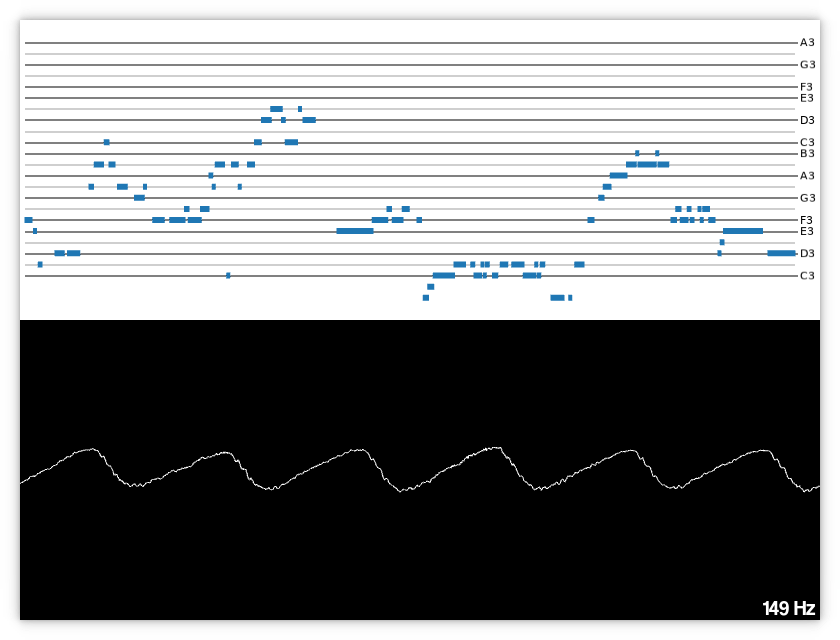
\includegraphics[width=.66\textwidth]{pictures/real-time.png}}
\end{center}
\end{frame}
\end{document}